% Name: TCP three-way handshake
% Description: A client and a server opening a TCP connection with SYN, SYN-ACK, and ACK, with the sequence numbers and each side's state as time runs down.
% Tags: TCP, handshake, networking, protocol

\usetikzlibrary{arrows.meta}

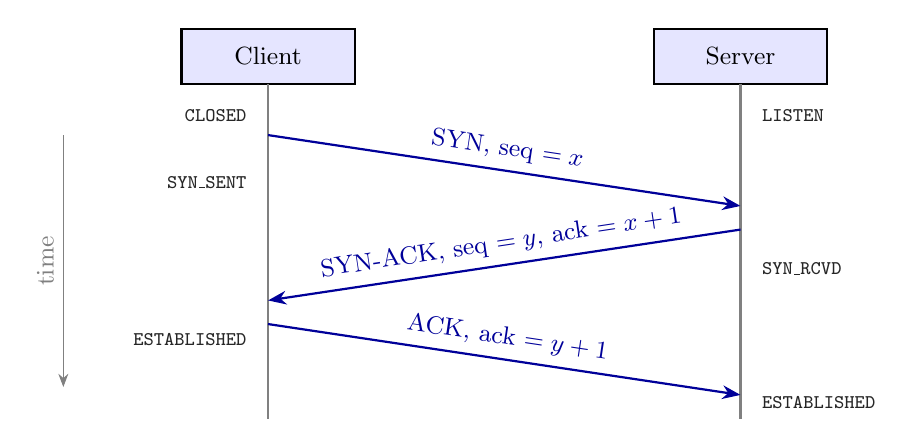
\begin{tikzpicture}[>={Stealth}, every node/.style={font=\small},
    host/.style={draw, thick, fill=blue!10, minimum width=22mm, minimum height=7mm},
    st/.style={font=\scriptsize\ttfamily, gray!30!black}, msg/.style={->, thick, blue!60!black}]
  \node[host] at (0,0) {Client};
  \node[host] at (6,0) {Server};
  \draw[thick, gray] (0,-0.35) -- (0,-4.6) (6,-0.35) -- (6,-4.6);
  % Each segment takes time to cross, so its arrow slopes down.
  \draw[msg] (0,-1) -- node[above, sloped] {SYN, seq $= x$} (6,-1.9);
  \draw[msg] (6,-2.2) -- node[above, sloped] {SYN-ACK, seq $= y$, ack $= x+1$} (0,-3.1);
  \draw[msg] (0,-3.4) -- node[above, sloped] {ACK, ack $= y+1$} (6,-4.3);
  \foreach \y/\s in {-0.75/CLOSED, -1.6/SYN\_SENT, -3.6/ESTABLISHED}
    \node[st, anchor=east] at (-0.15,\y) {\s};
  \foreach \y/\s in {-0.75/LISTEN, -2.7/SYN\_RCVD, -4.4/ESTABLISHED}
    \node[st, anchor=west] at (6.15,\y) {\s};
  \draw[->, gray] (-2.6,-1) -- node[left, rotate=90, anchor=south] {time} (-2.6,-4.2);
\end{tikzpicture}
